% !TEX root = ../main.tex
\section{Introduction}
\label{sec:intro}
Detection and identification using artificial landmarks has long been used in augmented reality and computer vision applications. Over the last decade, there has been numerous marker systems for obtaining more accurate detections and information encodings. Specifically, planar markers such as ARTag, ARToolkil, are among the most popular forms of fiducial markers.

Compared to markerless detection algorithms, these methods are simpler and produce much more reliable detections. There has been significant effort in improving the detection speed and encoding accuracy. They have yield great results for computer vision tasks that require high detection accuracies like camera calibrations, 3D reconstruction. Furthermore, they have gained popularity in the robotic community for having unique characteristics of high detection rates and numerous encoding schemes. For example, ARTags are commonly used to test SLAM systems or finding ground truth for objects in manipulation and motion planning tasks. 

Despite all the improvements in this field, obtaining accurate pose estimation from the tags remain a challenge. This is especially important for generalizing the use of fiducial tags in robotic applications. While current detection algorithm yield great results under well conditioned or simulated environments, it is very difficult to obtain reliable poses in noisy settings. For instances, when ARTags are used with low resolution camera or in poor lighting conditions, the system often produce poses with tremendous rotational errors as shown in Figure 2. In fact, we observe that the localization accuracy of the state of the art system perform significantly worse at difficult viewing angles or when there are noise in the scene. 

Based on the observation, we present two contributions in this paper. First, we conducted an in-depth analysis on the effect of various noises on pose estimation process. In particular, the noise in RGB images creates a perspective ambiguity problem that makes the pose estimation challenging without additional information. Second, we describe a novel algorithm that takes advantage of the RGBD sensors that are commonly available on most robotic systems to accurately estimate the pose from a single tag under noisy conditions. In the core of the algorithm, we recognize that depth data can produce good approximate initial pose in noisy scene. From the initial estimation, accurate poses can be calculated using constrained optimizations based on known uncertainty models of the sensor. There are few key features to this algorithm: 
\begin{itemize}
\item This method is highly robust to noise in the scene. It can obtain accurate poses suitable for robotic applications.   
\item It is easily generalizable to most fiducial tags designs.
\item It performs at worse as good as using only RGB images.
\end{itemize}

This paper also presents empirical results demonstrating the the successful performance of the algorithm on captured data from the robot. Our implementation of the algorithm is based off of the Apriltag detection pipeline and it is integrated with ROS. 

\begin{figure}
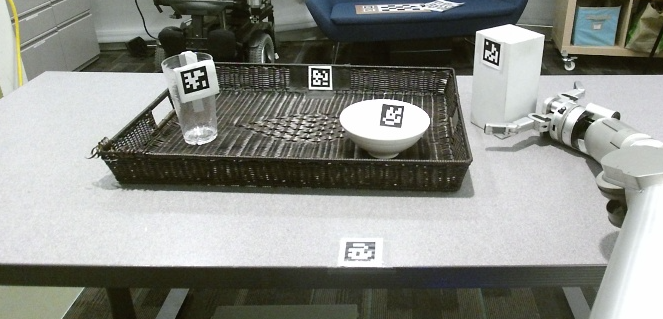
\includegraphics[width=\columnwidth, height=120px]{figs/table_clearing_rgb_small} \\
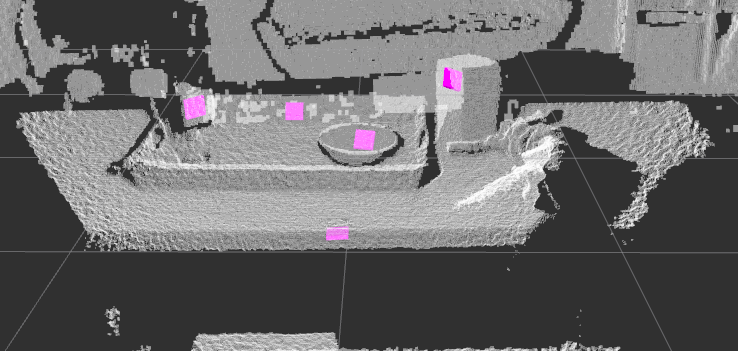
\includegraphics[width=\columnwidth, height=120px]{figs/table_clearing_depth}
\label{fig:table_clearing}
\caption{Apriltag used to localize objects in mainpulation tasks}
\end{figure}